
%
%  $Description: Author guidelines and sample document in LaTeX 2.09$ 
%
%  $Author: ienne $
%  $Date: 1995/09/15 15:20:59 $
%  $Revision: 1.4 $
%

\documentclass[times, 10pt,twocolumn]{article} 
\usepackage{latex8}
\usepackage{times}
\usepackage[german]{babel}
\usepackage[utf8]{inputenc}
\usepackage[T1]{fontenc}
\usepackage{listings}
\usepackage{hyperref}
\usepackage{breakurl}
\usepackage{color}
\usepackage{graphicx}

%for jDoc (begin)
\usepackage{ifthen}
\usepackage{arrayjob}
\makeatletter
\usepackage{trimspaces}
\usepackage{titlesec}
\def\trimspace#1{\trim@spaces@in{#1}}
\makeatother
\newarray\jDocArray

\readarray{jDocArray}{%
Number & java.lang.number & http://docs.oracle.com/javase/7/docs/api/java/lang/Number.html &%
Name & das.package.Ksasse & http://linkzujavadoc.de/path/path.html &%
AutoClosable & java.lang.AutoClosable & http://docs.oracle.com/javase/7/docs/api/java/lang/AutoCloseable.html &%
Connection & java.sql.Connection & http://docs.oracle.com/javase/7/docs/api/java/sql/Connection.html &%
Statement & java.sql.Statement & http://docs.oracle.com/javase/7/docs/api/java/sql/Statement.html &%
ResultSet & java.sql.ResultSet & http://docs.oracle.com/javase/7/docs/api/java/sql/ResultSet.html &%
Throwable & java.lang.Throwable & http://docs.oracle.com/javase/7/docs/api/java/lang/Throwable.html &%
END&X&X%
}
\dataheight=3

\newcommand{\jDocArrayValueCache}[2]{\checkjDocArray(#1,#2)\trimspace\cachedata}
\newcommand{\jDocArrayValue}[2]{\jDocArrayValueCache{#1}{#2} \cachedata}

\newcounter{jDocI}
\setcounter{jDocI}{1}

\jDocArrayValueCache{1}{1}
\whiledo{\not\equal{\cachedata}{END}}
{%
	\newboolean{jDoc\thejDocI} %Deklaration
	\setboolean{jDoc\thejDocI}{true} %Zuweisung
	\stepcounter{jDocI}%
	\jDocArrayValueCache{\thejDocI}{1}
}

\newcommand{\jd}[1]{%
	\setcounter{jDocI}{1}%
	\jDocArrayValueCache{1}{1}%
	\whiledo{\not\equal{\cachedata}{#1} \and \not\equal{\cachedata}{END}}%
	{%
		\stepcounter{jDocI}%
		\jDocArrayValueCache{\thejDocI}{1}%
	}%
	\ifthenelse{\equal{\cachedata}{END}}%
	{%
		\textbf{ERROR: could not find #1 in jDoc}%
	}%
	{%
		\ifthenelse{\boolean{jDoc\thejDocI}}%
		{%
			#1$_{java}$\footnote{\jDocArrayValue{\thejDocI}{2}\newline\tiny\jDocArrayValue{\thejDocI}{3}}%
			\setboolean{jDoc\thejDocI}{false}%
		}%
		{%
			#1$_{java}$%
		}%
	}%
}

\newcommand{\jDocIndex}{%
	%\begin{tabular}[h]{p{4cm}p{11.5cm}ll}%	
	\setcounter{jDocI}{1}%
	\jDocArrayValueCache{1}{1}%
	\whiledo{\not\equal{\cachedata}{END}}%
	{%
		\ifthenelse{\not\boolean{jDoc\thejDocI}}%
		{
			%Eintrag erstellen
			\begin{description}
				\item[\jDocArrayValue{\thejDocI}{1}]\jDocArrayValue{\thejDocI}{2} \linebreak
				\tiny\jDocArrayValue{\thejDocI}{3}
			\end{description}						
			%\jDocArrayValue{\thejDocI}{1} & \jDocArrayValue{\thejDocI}{2} \linebreak%
			%\tiny\jDocArrayValue{\thejDocI}{3} \\%
		}%
		{%
			%kein Eintrag erstellen
		}%
		\stepcounter{jDocI}%
		\jDocArrayValueCache{\thejDocI}{1}%
	}%
	%\end{tabular}%
}

%\jd{Test} \jd{Test} \jd{InputFormat}

%\jDocIndex
%for jDoc (end)

%Format Listings
\definecolor{javared}{rgb}{0.6,0,0} % for strings
\definecolor{javagreen}{rgb}{0.25,0.5,0.35} % comments
\definecolor{javapurple}{rgb}{0.5,0,0.35} % keywords
\definecolor{javadocblue}{rgb}{0.25,0.35,0.75} % javadoc

\lstset{language=Java,
basicstyle=\ttfamily,
keywordstyle=\color{javapurple}\bfseries,
stringstyle=\color{javared},
commentstyle=\color{javagreen},
morecomment=[s][\color{javadocblue}]{/**}{*/},
numbers=left,
numberstyle=\tiny\color{black},
stepnumber=1,
numbersep=10pt,
tabsize=4,
showspaces=false,
showstringspaces=false,
frame=single}


%------------------------------------------------------------------------- 
% take the % away on next line to produce the final camera-ready version 
\pagestyle{empty}

%------------------------------------------------------------------------- 
\begin{document}

\title{Sprachänderungen aus Java 7 - State of the Art}

\author{Jonas Traub\\
IBM Deutschland\\
Duale Hochschule Baden-Württemberg\\
jonas.traub@de.ibm.com
\and
Matthis Hauschild\\
IBM Deutschland\\
Duale Hochschule Baden-Württemberg\\
matthis.hauschild@de.ibm.com\\
}

\maketitle
\thispagestyle{empty}

\begin{abstract}
Dieses Dokument beschreibt den Stand der Technik der Java Programmiersprache mit besonderem Fokus auf die
Sprachänderungen, die mit dem Sprung auf Version 7 aus dem Jahr 2011 eingeführt wurden.\\

Für Java Entwickler bietet dieses State of the Art einen kompakten Einstieg in die neu geschaffenen Möglichkeiten und
behandelt gleichzeitig häufige Fehler, die den Einstieg in das Release erschweren.
\end{abstract}

\Section{Introduction}

Seit 2011 bietet Oracle mit Java 7 umfangreiche Erweiterungen, an der Programmiersprache im Vergleich zu den Vorgängerversionen, an.
Im Folgenden werden die wichtigsten Änderungen und Erweiterungen näher beschrieben. Neben Änderungen aus Project Coin,
wie der neue Diamond Operator, Binary literals und try-with-resources, wurden auch einige technisch
anspruchsvolle Neuerungen realisiert, die im Folgenden betrachtet werden. Hierzu zählen die neuen I/O Operationen aus NIO.2 und
das ForkJoin Framework.\\

An sinnvollen Stellen werden Codebeispiele verwendet, um die Sprachneuerungen zu verdeutlichen. Java Klassen sind durch die tiefgestellte
Markierung \textit{java} gekennzeichnet. Die zugehörigen Fußnoten verweisen auf die Java Documentation\cite{javadocs}. Eine 
vollständige Auflistung aller Neuerungen bietet Oracle in den Releasenotes zu Java 7\cite{oracleJavaRel} an.\\

Dieses Dokument soll mit den folgenden Kapiteln einen kurzen und prägnanten Überblick über Sprachänderungen aus Java 7 geben,
die im Arbeitsalltag besonders häufig relevant sind.

\Section{Diamond Operator}
Mit Java 5 wurden Generics in die Sprache eingeführt, die sich schnell großer Beliebtheit erfreut haben und von der Entwicklergemeinde sehr gut angenommen wurden. Nun, mit Java 7, hat Oracle die Deklaration von Variablen mit Generics deutlich vereinfacht.\cite{oracleJavaRel}\\

Noch in Java 6 musste der Typ in einer Deklaration mit Generics mehrfach angegeben werden.
\begin{lstlisting}[language=java,breaklines=true]
  List<Integer> name =
    new ArrayList<Integer>();
  Map<Integer,List<String>> name2 =
    new Map<Integer,List<String>>();
\end{lstlisting}
Java 7 unterstützt nun das automatische Rückschließen auf den deklarieren Datentyp bei der Initialisierung.\cite{v2bJava7} Statt der erneuten Angabe des Typs kann hier nun der Diamantoperator verwendet werden.
\begin{lstlisting}[language=java,breaklines=true]
  List<Integer> = new ArrayList<>();
  Map<Integer,List<String>> name2 =
    new Map<>();
\end{lstlisting}
Insbesondere bei verschachtelten Deklarationen ist dieses Feature in Verbindung mit der Autovervollständigung einer IDE sehr nützlich. Der Diamantoperator kann auch verwendet werden, wenn Initialisierung und Deklaration nicht in der selben Codezeile erfolgen.\cite{v2bJava7}\\

Auch die Verwendung in Verbindung mit dem Wildcardoperator wurde ermöglicht.
\begin{lstlisting}[language=java,breaklines=true]
  List<? extends Number> =
    new ArrayList<>();
\end{lstlisting}
Es wird hier bei der Initialisierung immer auf den allgemeinst möglichen Typ zurück geschlossen. Im konkreten Beispiel also auf \jd{Number}.\cite{v2bJava7}

\Section{try-with-resources}\label{try_sec}
Neu mit Java 7 ist das Automatic Resource Management\cite{javainsel2}, oft auch \texttt{try-with-resources} genannt, was die normale try-catch-finally 
Routine erweitert, um die beiden folgenden Probleme zu adressieren:
\begin{enumerate}
\item Das Schließen einer Ressource benötigt oft ein zusätzliches try-catch
\item Eine Exception im finally-Block überdeckt eine etwaige Exception aus dem try-Block
\end{enumerate}

Mit Ressourcen sind hier alle Klassen gemeint, die die neue Schnittstelle \jd{AutoClosable} implementieren, wie beispielsweise
InputBuffer- und OutputBuffer-Klassen, aber auch die JDBC-Klassen \jd{Connection}, \jd{Statement} und \jd{ResultSet}.

Um \texttt{try-with-resources} nutzen zu können, wird die Syntax des \texttt{try}s um einen Anweisungsblock in runden Klammern erweitert,
in dem nun alle, am Ende zu schließenden, Ressourcen initialisiert werden. Das folgende Beispiel illustriert den Unterschied zwischen der
klassischen Variante des manuellen Schließens der geöffneten Ressourcen, sowie der neuen Variante mit \texttt{try-with-resources}:

\begin{lstlisting}[language=java,breaklines=true]
Connection con = null;
Statement stmt = null;
ResultSet rs = null;

try {
  con = DriverManager.getConnection(
	"jdbc:hsqldb:file:/tmp/hsql;shutdown=true", "root", "");
  stmt = con.createStatement();
  rs = stmt.executeQuery(
    "SELECT * FROM Customer" );
  while (rs.next()) {
	System.out.printf("%s, %s%n", rs.getString(1), rs.getString(2));
  }
} catch (SQLException e) {
  e.printStackTrace();
} finally {
  try {
	if (rs != null) rs.close();
  } catch (SQLException e) {
	e.printStackTrace();
  } finally {
	try {
	  if (stmt != null)	stmt.close();
	} catch (SQLException e) {
	  e.printStackTrace();
	} finally {
	  try {
		if (con != null) con.close();
	  } catch (SQLException e) {
		e.printStackTrace();
} } } }
\end{lstlisting}

Es ist zu erkennen, dass, um alle drei Ressourcen sicher schließen zu können, drei ineinander verschachtelte try-catch-finally Blöcke
gebraucht werden. Ein weiterer Nachteil dieser Lösung ist das Unterdrücken einer Exception, wenn gleichzeitig in Zeile 2 sowie in einer
der \texttt{close()}-Methoden eine Exception geworfen wird. Dann überdeckt die Exception der \texttt{close()}-Anweisung die andere und der
Anwender bekommt sie niemals zu Gesicht.\cite{javainsel2}

\begin{lstlisting}[language=java,breaklines=true]
try (
  Connection con = DriverManager.getConnection(
	"jdbc:hsqldb:file:/tmp/hsql;shutdown=true", "root", ""
  );
  Statement stmt = con.createStatement();
  ResultSet rs = stmt.executeQuery(
    "SELECT * FROM Customer");
) {
  while (rs.next()) {
	System.out.printf("%s, %s%n", rs.getString(1), rs.getString(2));
  }
} catch (SQLException e) {
  e.printStackTrace();
}
\end{lstlisting}

Bei \texttt{try-with-resources} kann man alle Ressourcen, die \jd{AutoClosable} implementieren, mit Semikola getrennt 
nach dem \texttt{try} auflisten. Damit werden sie automatisch am Ende des Blocks geschlossen und falls mehrere Exceptions auftreten,
werden alle an den Anwender hochgereicht. Wie das genau gemacht wird, wird in Kapitel \ref{supp_exception_subsec} erläutert. 

\Section{Literals}
\SubSection{Binary Literals}

Während in der bisherigen Javaversion 6 Zahlenliterale nur in oktaler, dezimaler und hexadezimaler angabeform möglich waren, erlaubt java 7 nun auch Binäre literale. Binäre Literale können mit dem Präfix \texttt{0b} geschrieben werden.

Insbesondere bei der Angabe negativer Zahlen ist jedoch Vorsicht geboten. Für die Datentypen \texttt{byte} und \texttt{short} kann das erste Bit nicht direkt angegeben werden. Es sind also nur 7 bzw. 15 statt 8 und 16 Bit lange Angaben möglich. Die Angabe ob es sich um eine Negative Zahl handelt erfolgt hier durch ein Minuszeichen. Zu beachten ist jedoch, dass der Wert der Binärzahl dadurch negativ dargestellt wird. Dies ist nicht Äquivalent mit einer Invertierung des Vorzeichenbits, was Zeilen 1-3 des folgenden Beispiels verdeutlichen.\cite{sbJ7literals}
\begin{lstlisting}[language=java,breaklines=true]
  byte zahl1 =  0b1111111  // 127
  byte zahl2 = -0b1111111  //-127
  byte zahl3 = -0b10000000 //-128
  byte zahl4 =  0b01111111 // 127
  byte zahl5 =  0b10000000 //ERROR
\end{lstlisting}
Auffallend ist nun noch dass führende Nullen ignoriert werden (Zeile 4), wenn hingegen ein gleich langes Literal den Wertebereich des Datentyps überschreitet führt dies zu einem Compilererror (Can not convert from int to byte)\cite{sbJ7literals}.\\

Beim Datentyp \texttt{int} gelten inkonsistenter Weise andere Regeln. Werden bei einem \texttt{int} die vollen 32 Bit angegen, wird das linkeste Bit als Vorzeichenbit interpretiert. Es kommt nicht zu einem Compilererror. Die zusätzliche Angabe den Minus Vorzeichens führt jedoch auch hier zu einer direkten Negativdastellung des Zahlenwerts und nicht zur Invertierung der des Vorzeichenbits. Erst ab dem 33 Bit kommt es zu einem Compilererror (out of range).
\begin{lstlisting}[language=java,breaklines=true]
int i=
 0b1000000000000000_0000000000000000;
 //-2147483648
int j=
 -0b1000000000000000_0000000000000000;
 //-2147483648
int k=
 0b1010101010101010_1010101010101010;
 //-1431655766
int l=
 -0b1010101010101010_1010101010101010;
 // 1431655766
int m=
 0b0010101010101010_1010101010101010;
 // 715827882
int n=
 -0b0010101010101010_1010101010101010;
 //-715827882
\end{lstlisting}

Verwunderlich ist hier zunächst das zweite Beispiel. Trotz des zusätzlichen Vorzeichens ist das Erbegnis identisch. Das Vorzeichen negiert den Zahlenwert. Erwarten würden wir also das Ergebnis \texttt{2147483648}. Da dies jedoch außerhalb des Wertebereichs von \texttt{int} liegt kommt ein Overflow um \texttt{1} hinzu. Ergebnis ist somit wieder \texttt{-2147483648}.\\

Literale des Datentyps \texttt{long} werden wie gewohnt mit einem \texttt{L} oder \texttt{l} am Ende des Literals kenntlich gemacht (z.B. \texttt{0b1010L}). Gleitkommazahlen können \textbf{nicht} als binäre Literale angegeben werden. Die Endungen \texttt{D}, \texttt{d}, \texttt{F} und \texttt{f} führen folglich zu einem Compiler Error.

\SubSection{Underscores in Numeric Literals}
Zur Verbesserung der Übersichtlichkeit ermöglich Java 7 die Notation von Unterstrichen in Zahlenliteralen. Unterstriche sind nur an Position zwischen zwei Ziffern zulässig, also nicht am Anfang oder Ende des Literals, nicht vor oder nach Datentypangaben oder Literaltypangaben und nicht Angrenzend an das Dezimaltrennzeichen (\texttt{.}).\cite{apressjava} An den zulässigen Positionen können beliebig viele Unterstriche aufeinander folgen.\cite{heiseWasistNeu}

\begin{lstlisting}[language=java,breaklines=true]
int   i=0b_001;  //invalid
int   j=123_L;   //invalid
int   k=_123;    //invalid
int   l=123_;    //invalid
float m=12._34;  //invalid
int   n=1____2;  //valid
float o=1_2.3_4; //valid
\end{lstlisting}

\Section{Strings in switch Statements}
Eine weitere Neuerung aus Java 7 ist die Möglichkeit, das \texttt{switch} Statement auch mit Strings zu verwenden, statt wie
zuvor nur mit Ganzzahldatentypen kompatibel zu \texttt{Integer} (char, byte, short, int). Dabei kann nun direkt ein String
angegeben werden, oder auf eine zur Compile-Zeit bekannte Konstante zurückgegriffen werden. Nicht möglich ist die Verwendung
von Regexen oder der Abfrage auf \texttt{null}.\cite{javainsel2}

\begin{lstlisting}[language=java,breaklines=true]
String str1 = "TWA";
final String STR2 = "DB";

switch (str1) {
case "CTV": //valid
case STR2:  //valid
case null:  //Compiler-Error
case 42:	//Compiler-Error
}
\end{lstlisting}

\Section{Varargs mit Generics}
Um die in diesem Abschnitt vorgestelleten Verbesserungen verstehen zu können ist zunächst die Feststellung von Bedeutung, dass Java laut Sprachdefinition keine Arrays aus generischen Datentypen erlaubt.
\begin{lstlisting}[language=java,breaklines=true]
int i[]=new int[500]; //is valid, but
//the following causes a compiler error
List<String> j[]=new List<String>[500];
\end{lstlisting}
Es können jedoch durchaus generische Datentypen in Varargs verwendet werden. Der Methodenkopf \texttt{void myMethod(List<String>... x)} ist somit gültig. Die übergebenen Listen werden innerhalb der Methode als Array mit dem Namen \texttt{x} repräsentiert. Da ein Array aus \texttt{list<String>} jedoch nicht möglich ist erhalten wir nur ein Array vom Typ \texttt{List}. Die generische Typisierung geht also verloren.\\

Die führt dazu, dass der Compiler nicht mehr überprüfen kann, ob die Elemente des Arrays aus dem Parameter \texttt{x} auch typsicher verwendet werden.\cite{v2bJava7}\\

Der Java 6 Compiler liefert im beschriebenen Fall nur eine Warning beim Aufruf der Methode (\texttt{uses unchecked or unsave operations} bzw. \texttt{unchecked generic array creation}), nicht jedoch bei deren Deklaration. Es werden also nur die Nutzer und nicht der Autor einer Methode vor dem eventuellen Problem der Typunsicherheit gewarnt.\\

Der Java 7 Compiler unterstützt den Entwickler nun mit einer zusätzlichen Warnung (\texttt{possible heap pollution}) die an der Postion der Methodendeklaration erzeugt wird.\\

Um die Warnungen bei den Methodenaufrufen in Java 6 zu unterdrücken musste bei jedem Aufruf ein 
%geschachteltes texttt, weil "u sonst zu ü wird. Known bug in german option.
\texttt{@SuppressWarnings(}"\texttt{unchecked}"\texttt{)} eingefügt werden. In Java 7 erlaubt nun die neue Annotation \texttt{@SafeVarargs} dem Autor einer Methode das unterdrücken aller genannten Warnings aufeinmal. Die Annotation muss dafür nur bei der Deklaration angegeben werden und wirkt sich dann auch auf die Warnings bei Aufrufen der Methoden unterdrückend aus.

\Section{Exceptions}
\SubSection{Catch Multiple Exceptions at once}
Desöfteren wirft ein Code Fragment mehrere Exceptions, die zwar unterschiedliche Ursachen haben, aber dennoch gleich behandelt
werden sollen. Ein Szenario wäre die Klasse \jd{Scanner} zu verwenden, um eine Datei einzulesen. Dabei könnten eine 
\texttt{IOException} beim fehlerhaften Öffnen der Datei sowie eine \texttt{InputMismatchException} beim Parsen auftreten.

Angenommen, es sollen sehr viele Dateien geparsed und eine fehlerhafte Datei einfach übersprungen werden, 
gleich welcher Fehler auftritt, könnten zwei \texttt{catch} Blöcke verwendet werden, die beide redundanten Code enthalten.
\begin{lstlisting}[language=java,breaklines=true]
try {/*...*/} 
catch (InputMismatchException e) {
	/* parse next file */}
catch (IOException e) {
	/* parse next file */}
\end{lstlisting} 
Dies sorgt natürlich für unnötige Code-Duplizierung, was zu Fehlern führen könnte, wenn das Verhalten nachträglich geändert 
werden soll, dabei aber ein \texttt{catch} Block vergessen wird.

Was deshalb gerne gemacht wird, ist die generelle \texttt{Exception} abzufangen.
\begin{lstlisting}[language=java,breaklines=true]
try {/*...*/} 
catch (Exception e) {
	/* parse next file */}
\end{lstlisting}
Ein Nachteil, der im ersten Moment gerne vergessen (oder bewusst ignoriert) wird, ist, dass dieser \texttt{catch} Block 
\textbf{alle} Exceptions abfängt, eben auch \texttt{RuntimeException}s. Dies ist oft ein unterwünschtes Verhalten, da 
beispielsweise \texttt{NullPointerException}s oft ein Indikator für fehlerhaften Code sind und dies nicht mehr auffälle,
wenn nun einfach die Datei übersprungen und mit der nächsten fortgefahren würde.

Die mit Java 7 eingeführte Lösung des Problems nennt sich \texttt{Multi-catch}. Dabei ist es möglich, mehrere Exceptions
mit nur einem \texttt{catch} Block abzufangen. Dazu werden alle abzufangenen Exceptions mit einer Pipe (|) verbunden.\cite{javainsel2}
\begin{lstlisting}[language=java,breaklines=true]
try {/*...*/} 
catch (InputMismatchException | IOException e) {
	/* parse next file */}
\end{lstlisting}
Hierbei ist es wichtig zu erwähnen, dass \texttt{e} dadurch \texttt{final} wird, also seine Referenz im \texttt{catch} Block 
nicht mehr verändert werden darf. Des Weiteren ist es auch nicht möglich, Exceptions aus dem selben Zweig hintereinander
zu hängen. So ist es beispielsweise nicht möglich, \texttt{IOException} und \texttt{FileNotFoundException} zu kombinieren,
weil letztere eine Subklasse von ersterer ist. Dies ist auch nicht möglich, wenn die \texttt{FileNotFoundException} zuerst
genannt wird, wie es bei der klassischen Methodik vom Fangen mehrerer Exceptions der Fall ist.

\SubSection{Rethrow Exceptions}
Dieses Feature adressiert den Wunsch der Entwicklergemeinde weniger unnötigen und redundanten Java Code schreiben zu müssen.\cite{sbJ7exeptions}\\

Häufig kommt es vor, dass eine Exception in einem \texttt{try} Block auftritt, dann in einem \texttt{catch} Block abgefangen und bearbeitet wird und schließlich dennoch durch einen erneuten \texttt{throw} Befehl an die aufrufende Methode hochgereicht wird.

\begin{lstlisting}[language=java,breaklines=true]
public static void main(String args[]) throws Exception {
    boolean flag = true;
    try {
        if (flag){
            throw new OpenException();
        }
        else {
            throw new CloseException();
        }
    }
    catch (Exception e) {
        System.out.println(e.getMessage());
        throw e;
    }
}
\end{lstlisting}

Obiger Code\cite{sbJ7exeptions} zeigt eine Möglichkeit dies mit Java 6 zu realisieren. Es wird im \texttt{catch} Block die allgemeine \jd{Exception} Klasse statt der tatsächlichen erbenden \texttt{Open}- bzw. \texttt{CloseException} abgefangen. Hierdurch kommt es jedoch auch zu einer Verallgemeinerung der \texttt{throws} Deklaration der Methode auf \jd{Exception} und die detailliertere Typisierung geht beim rethrow verloren. Dieses Problem konnte noch in Java 6 nur umgangen werden in dem getrennte \texttt{catch} Blöcke mit redundantem Code für jede Exception verwendet wurden. Alternativ musste der Code zum Exceptionhandling in eine externe Methode ausgelagert werden, die dann in getrennten \texttt{catch} Blöcken aufgerufen wurde.\cite{scjp6}\\

In Java 7 erkennt der Compiler nun, welche checked Exceptions tatsächlich im \texttt{try} Block geworfen werden können. Ebenso erkennt der Compiler wenn es sich um einen rethrow einer Exception hadelt. Mit Java 7 kann dadurch der Methodenkopf im obigen Beispiel mit expliziten Exceptions angegeben werden ohne, dass es zu einem Copiler Error kommt\cite{sbJ7exeptions}.

\begin{lstlisting}[language=java,breaklines=true]
public static void main(String args[]) throws OpenException, CloseException
\end{lstlisting}

Dieses Feature kann problemlos in Kombination mit dem Multicatch Feature verwendet werden.

\SubSection{Suppressed Exceptions}\label{supp_exception_subsec}
Suppressed Exceptions wurden eingeführt, um das, in Java 7, neu auftretende Problem von \texttt{try-with-resources} zu adressieren.
Mit dem neuen Konstrukt ist es nämlich möglich, dass zwei Exceptions gleichzeitig auftreten können (siehe Kapitel \ref{try_sec}), wenn im
\texttt{try}-Block sowie in der automatisch aufgerufenen \texttt{close()}-Methode jeweils eine Exception geworfen wird. Dies würde
dazu führen, dass die Hauptexception unterdrückt würde und der Anwender lediglich die Exception vom \texttt{close()} bekommen würde.

Suppressed Exceptions bieten nun die Möglichkeit, eine Exception an eine andere heranzuhängen, um so beide an den Anwender zu
kommunizieren. Dafür wurde die Klasse \jd{Throwable} um die beiden Methoden 
\begin{lstlisting}[language=java,breaklines=true]
public final void addSuppressed(Throwable exception)
\end{lstlisting}
und 
\begin{lstlisting}[language=java,breaklines=true]
public final Throwable[] getSuppressed()
\end{lstlisting}
erweitert, um die Exceptions anzuhängen und wieder abgreifen zu können. 
Bei \texttt{try-with-resources} braucht sich der Programmierer um das Schachteln nicht zu kümmern, dies wird 
automatisch vom Compiler erledigt.\cite{sbJ7coin} Lediglich bei der Abarbeitung der Exceptions kann er nun über
alle Exceptions iterieren und entsprechenden Code ausführen lassen. Bei Verwendungen der Methode
\begin{lstlisting}[language=java,breaklines=true]
public void printStackTrace()
\end{lstlisting}
aus der Klasse \jd{Throwable} werden automatisch alle unterdrückten Exceptions mit angegeben. Eine Beispielausgabe dazu könnte
folgendermaßen aussehen\cite{javainsel2}:
\begin{lstlisting}[language=java,breaklines=true]
Exception in thread "main" java.lang.NullPointerException
  at SuppressedClosed.main(SuppressedClosed.java:14)
  Suppressed: java.lang.UnsupportedOperationException: close() mag ich nicht
    at SuppressedClosed$1NotClosable.close(SuppressedClosed.java:9)
    at SuppressedClosed.main(SuppressedClosed.java:15)
\end{lstlisting}

Es ist zu erkennen, dass die Hauptexception eine \texttt{NullPointerException} ist und eine unterdrückte 
\texttt{UnsupportedOperationException} angefügt wurde (Zeile 3).

\Section{NIO.2}
Mit Java 7 wurde das im Jahre 2002 mit Java 1.4 eingeführte NIO (new Input/Output) verbessert und in einer Version NIO.2
herausgegeben.\cite{v2bJava7} NIO.2 umfasst viele Änderungen, wobei hier auf die wichtigsten bezüglich Dateien und
Dateisystemen eingegangen wird.

Alle vorgestellten Klassen sind im Package \texttt{java.nio} zu finden.

\SubSection{Einfache Datei- und Pfadoperationen}
Neu hinzugekommen ist die Klasse \jd{Path}, welche viele Methoden zum Erstellen und Modifieren von Dateisystempfaden enthält. Dabei ist
wichtig zu erwähnen, dass die Klasse nicht wirklich auf dem Dateisystem arbeitet, sondern die Pfade nur repräsentiert. Zum tatsächlichen
Modifizieren wird beispielsweise die Hilfsklasse \jd{Files} verwendet. Die Pfade sind über viele Methoden veränderbar und dies ist auf
allen Betriebssystemen einheitlich. Trotzdem sind die Path-Objekte betriebssystemabhängig, da sie letztenendes Pfade 
im Dateibaum darstellen.
\begin{lstlisting}[language=java,breaklines=true]
Path p1 = 
  Paths.get("test/a", "aa/dok1.txt");
Path p2 = Paths.get("test/b/");

p2.relativize(p1); // ..\a\aa\dok1.txt
p1.toAbsolutePath(); 
// C:\Users\Matthis\test\a\aa\dok1.txt
p2.getName(0); // test
\end{lstlisting}
Hier sind beispielhaft einige Methoden von \jd{Path} benutzt worden. Um einen Pfad zu erstellen, kann die 
Methode \texttt{static Path get(String first, String... more)} aus der Hilfsklasse \jd{Paths} verwendet werden.

\jd{Path} bietet Möglichkeiten, um einen Pfad von einem zu einem anderen zu bilden, einen absoluten Pfad zu erstellen,
einzelne Teile aus einem Pfad zu extrahieren, das Elternelement zurückzugeben und viele mehr.

Um nun tatsächlich Änderungen im Dateisystem durchführen zu können, kann die oben erwähnte Klasse \jd{Files} verwendet werden.
Diese bietet Unterstützung für einfache Operationen wie Verschieben, Kopieren und Löschen, kann aber auch Dinge, die früher
mit \jd{File} nur schwierig zu realisieren waren, wie Datei-Attribute verändern, symbolische und harte Links erstellen oder
direkt einen geöffneten Stream auf eine Datei zurückgeben.\cite{b247nio2}
\begin{lstlisting}[language=java,breaklines=true]
Path p1 = 
 Paths.get("test/a", "aa/dok1.txt");
Path p2 = 
 Paths.get("test/b/kopierteDatei.txt");

Files.isRegularFile(p1); //true
Files.getLastModifiedTime(p1); 
//2013-03-04T15:25:52.53087Z
Files.copy(p1, p2); 
//erzeugt neue Datei kopierteDatei.txt
Files.createSymbolicLink(
  Paths.get("test/link.lnk"), p1);

try (BufferedReader in = 
  Files.newBufferedReader(p1, Charset.defaultCharset())) {
	System.out.println(in.readLine());
}
\end{lstlisting}
Wie man sehen kann, sind die neuen Methoden sehr einfach zu benutzen und erleichtern das Handling mit Dateien besonders,
wenn eine Applikation für verschiedene Betriebssysteme geschrieben wurde.

\SubSection{Verzeichnis-Operationen}
Ein weiteres Konzept ist der \jd{FileVisitor}. Oft möchte man durch einen Verzeichnisbaum iterieren und auf jede Datei eine
Operation durchführen.
Der Methode \texttt{static Path walkFileTree(Path start, FileVisitor<? super Path> visitor)} aus \jd{Files} kann man einen
FileVisitor mitgeben. Sie iteriert dann rekursiv über den angegebenen Pfad und wendet die Operationen des FileVisitors an.

Ein FileVisitor muss folgende Methoden implementieren:
\begin{itemize}
  \item preVisitDirectory()
  \item visitFile()
  \item visitFileFailed()
  \item postVisitDirectory()
\end{itemize}
Diese stellen die Möglichkeiten zur Verfügung, beim Iterieren sehr feingranular Operationen auszuführen, so dass man nicht nur auf jeder
Datei (\texttt{visitFile}), sondern auch beim Eintritt (\texttt{preVisitDirectory}) und Austritt (\texttt{postVisitDirectory})
aus einem Verzeichnis, sowie im Fehlerfall (\texttt{visitFileFailed}) eine Aktion ausführen lassen kann.

Den Iterationsprozess kann man durch Rückgabewerte der zuvor genannten Operationen beeinflussen mit
\begin{itemize}
  \item CONTINUE\\
  Zur nächsten Datei gehen
  \item TERMINATE\\
  Iteration abbrechen
  \item SKIP\_SUBTREE\\
  Dieses Unterverzeichnis überspringen
  \item SKIP\_SIBLINGS\\
  Alle Verzeichnisse auf gleicher Ebene überspringen
\end{itemize}
aus der Enumeration \jd{FileVisitResult}.

Das folgende Beispiel zeigt die Ausgabe des Dateinamens jeder vorhandenen Datei in einem Verzeichnis mit Hilfe des
\jd{SimpleFileVisitor}s, einer Klasse, die das \jd{FileVisitor}-Interface bereits vorimplementiert, sodass nur noch die
benötigten Methoden (hier \texttt{visitFile}) überschrieben werden müssen:
\begin{lstlisting}[language=java,breaklines=true]
Path p1 = 
  Paths.get("test/a", "aa/dok1.txt");

Files.walkFileTree(p1.getName(0), 
  new SimpleFileVisitor<Path>() {
	@Override
	public FileVisitResult visitFile(Path file, BasicFileAttributes attrs) throws IOException {
      System.out.println(file);
      return FileVisitResult.CONTINUE;
	}
});
\end{lstlisting}

\SubSection{Verzeichnisse im Dateisystem ueberwachen}
Java 7 bietet die Möglichkeit, komfortabel Verzeichnisse in einem Dateisystem auf bestimmte Änderungen zu überwachen.
Dies wird über einen \jd{WatchService}s realisiert. Dabei kann ein WatchService auf ein bestimmtes Verzeichnis registriert
werden. Es ist möglich, zu bestimmen, bei welchen Operationen ein Event kreiert werden soll.
\begin{itemize}
  \item ENTRY\_CREATE
  \item ENTRY\_DELETE
  \item ENTRY\_MODIFY
\end{itemize}
sind die drei vorhandenen Arten aus der Klasse \jd{StandardWatchEventKinds}.

Das folgende Beispiel illustriert die Registrierung eines WatchServices auf das Verzeichnis \texttt{test/b/} aus den vorherigen
Beispielen und überwacht dabei, ob eine neue Datei angelegt wurde.
\begin{lstlisting}[language=java,breaklines=true]
Path p2 = Paths.get("test/b/");

WatchService ws = FileSystems.getDefault().newWatchService();
WatchKey wk = p2.register(ws, StandardWatchEventKinds.ENTRY_CREATE
);

try{
  WatchKey watchKey = ws.poll(60,TimeUnit.SECONDS);
  List<WatchEvent<?>> events = wk.pollEvents();
  for(WatchEvent<?> event : events)
    System.out.println("Datei erstellt");
}catch(InterruptedException e){
  Thread.currentThread().interrupt();
}
\end{lstlisting}

Insgesamt bringt NIO.2 viele Neuerungen mit, die den Programmierer mit plattformübergreifenden Möglichkeiten zur einfachen
Manipulation von Dateien und Verzeichnissen ausstatten. 

\Section{ForkJoin-Framework}
Bereits in Java 5 wurde mit dem \jd{ThreadPoolExecutor} eine zentrale Eingangs-\jd{Queue} für neue Tasks (\jd{Runnable} oder \jd{Callable}) etabliert, die alle Worker Threads gemeinsam nutzen. Nun gibt es mit Java 7 eine weitere Implementierung von \jd{AbstractExecutorService}. Sie basiert auf dem Konzept des Fork/Join Frameworks\cite{forkjoinpaper} von Doug Lea.\cite{forkjoinheise}\\

Das ForkJoin-Framework ermöglich dabei eine besonders effektive Bearbeitung von Algorithmen, die nach dem Teile-und-Hersche-Verfahren funktionieren. Eine weitere Anwendungsmöglichkeit sind MapReduce Anwendungen.\\

\begin{figure}[h!]
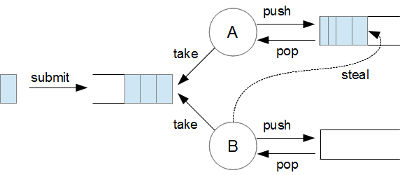
\includegraphics[width=8cm]{../images/forkjoin.png}
\caption[Fork/Join Image.]{Ein ForkJoinPool mit zwei Worker Threads A und B. Neben der Eingangs-\jd{Queue} existiert zusätzlich eine weitere interne Task \jd{Queue} pro Thread. Jeder Thread arbeitet zunaechst die eigene \jd{Queue} ab, bevor er sich einer anderen zuwendet. Quelle: Heise Developer\cite{forkjoinheise}}
\label{forkjoinpic}
\end{figure}

Abbildung \ref{forkjoinpic} zeigt die Funktionsweise des ForkJoin Framworks. Auch hier gibt es einen Threadpool mit einer zentralen Taskqueue. Im Gegensatz zu den Threadpools früherer Java Versionen hat hier jedoch jeder Thread zusätzlich eine eigene lokale \jd{Queue}, die dieser zuerst abarbeitet. Erst wenn diese leer ist greift der Thread auf die Queues anderer Threads im Pool zu. Nur wenn dies ebenfalls nicht mehr möglich ist bezieht er neue Aufgaben aus der Hauptqueue.\\

Durch dieses Vorgehen kann jeder Thread möglichst lange auf der eigenen lokalen \jd{Queue} arbeiten, die intern nun als performantere \jd{Deque} (double-ended queue) realisiert ist. Werden keine Tasks mehr aufgefunden wird der Thread pausiert und bei neuen Tasks von der JVM gezielt wieder angesprochen.\cite{forkjoinheise}\\

\bibliographystyle{latex8}
\bibliography{../stateofart}

\jDocIndex

\end{document}

